\documentclass[professionalfonts]{beamer}
\usetheme[numbering=fraction,progressbar=foot]{metropolis}
\usepackage{FiraSans}
\usepackage{graphicx}
\usepackage{color}
\usepackage{appendixnumberbeamer} 

\setbeamercolor{background canvas}{bg=white}
\setlength{\parskip}{1em}

\newcommand{\clr}{\operatorname{clr}}
\newcommand{\N}{\operatorname{Normal}}
\newcommand{\cov}{\operatorname{cov}}
\newcommand{\var}{\operatorname{var}}

\DeclareMathOperator*{\argmax}{arg\,max}
\DeclareMathOperator{\tr}{tr}

\title{Covariance Properties and Graph Selection for High-Dimensional Compositional Data}
\author{Camden Lopez}
\date{WNAR 2017, Student Paper Session 3}

\begin{document}

\maketitle

\begin{frame}{Outline}
\begin{itemize}
\item Compositional microbiome data
\item Graphical model selection using SPIEC-EASI
\item Covariance relationships and properties
\item Graph selection performance
\end{itemize}
\end{frame}

\begin{frame}{Compositional microbiome data}
16S amplicon sequencing
\begin{itemize}
\item Sample $\rightarrow$ DNA $\rightarrow$ 16S sequences $\rightarrow$ OTU counts
\item \textbf{Relative abundances only}
\end{itemize}
\begin{center}
\begin{tabular}{r|cccc}
& OTU 1 & OTU 2 & $\dots$ & OTU $p$ \\
\hline
Sample 1 & 136 & 28 & $\dots$ & 10 \\
Sample 2 & 0 & 2 & $\dots$ & 18 \\
$\vdots$ & $\vdots$ & $\vdots$ & $\ddots$ & $\vdots$ \\
Sample $n$ & 54 & 25 & $\dots$ & 5
\end{tabular}

OTU = operational taxonomic unit
\end{center}
\end{frame}

%\begin{frame}{Graphical model inference using SPIEC-EASI}
%\textbf{SP}arse \textbf{I}nvers\textbf{E} \textbf{C}ovariance Estimation for \\ \textbf{E}cological \textbf{AS}sociation \textbf{I}nference (Kurtz et al. 2015)
%
%Infers \textbf{graphical model} representation of OTU log abundances $\log W = (\log W_1, \dots, \log W_p)$
%\begin{columns}
%\begin{column}{0.6\textwidth}
%\begin{center}
%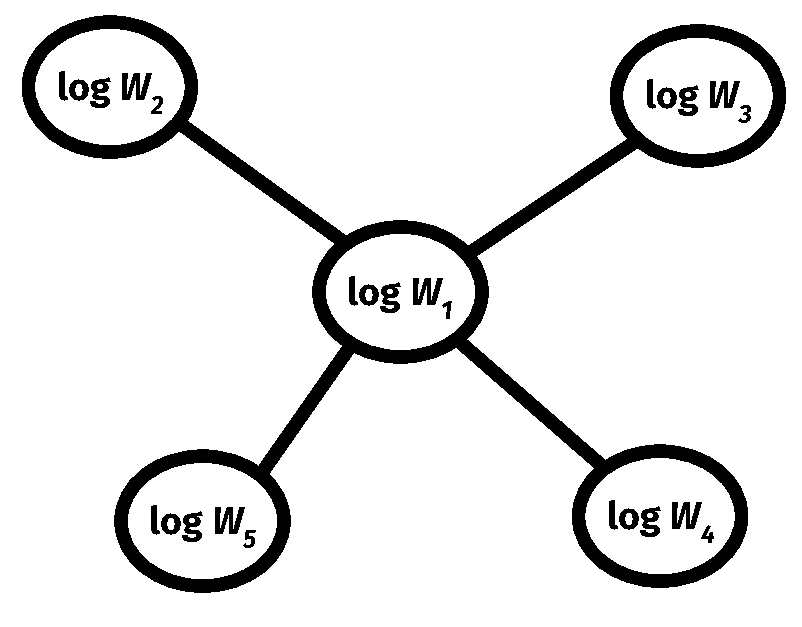
\includegraphics[width=150px]{figs/graph-model-log.pdf}
%\end{center}
%\end{column}
%\begin{column}{0.4\textwidth}
%based on \textbf{non-zero entries of $\Omega^{-1}$}, where $\Omega = \cov(\log W)$
%\end{column}
%\end{columns}
%\end{frame}

\begin{frame}{Graphical model inference using SPIEC-EASI}
\textbf{SPIEC-EASI}: \textbf{SP}arse \textbf{I}nvers\textbf{E} \textbf{C}ovariance Estimation for \\ \textbf{E}cological \textbf{AS}sociation \textbf{I}nference (Kurtz et al. 2015)
\begin{columns}
\begin{column}{0.6\textwidth}
\begin{itemize}
\item Relationships among OTU abundances $W = (W_1, \dots, W_p)$?
\item Suppose $\log W \sim \N(\,\cdot\,, \Omega)$
\item \textbf{Non-zero entries of $\Omega^{-1} \Leftrightarrow$ \\ conditional dependence, graphical model}
\end{itemize}
\end{column}
\begin{column}{0.4\textwidth}
\begin{center}
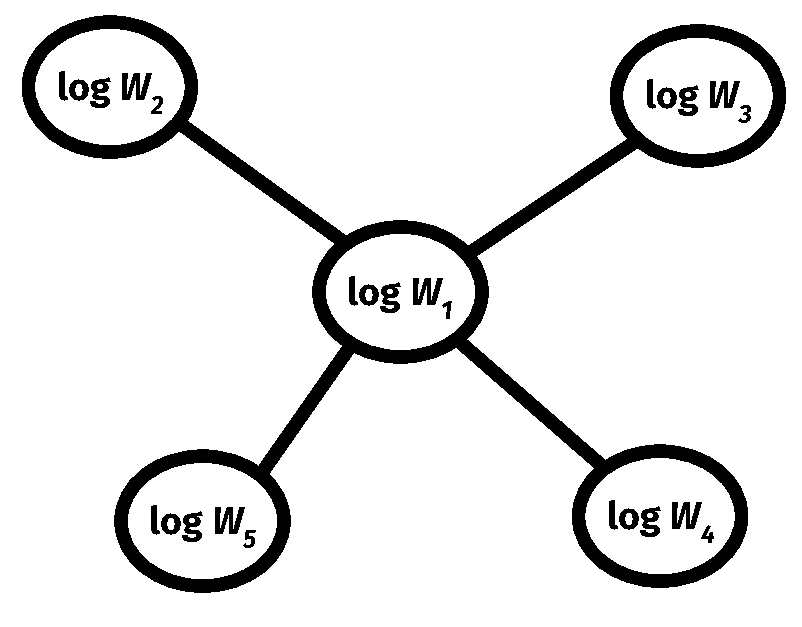
\includegraphics[width=110px]{figs/graph-model-log.pdf}
\end{center}
\end{column}
\end{columns}
\end{frame}

\begin{frame}{Graphical model inference using SPIEC-EASI}
\textbf{SPIEC-EASI}: \textbf{SP}arse \textbf{I}nvers\textbf{E} \textbf{C}ovariance Estimation for \\ \textbf{E}cological \textbf{AS}sociation \textbf{I}nference (Kurtz et al. 2015)
\begin{columns}
\begin{column}{0.6\textwidth}
\begin{itemize}
\item \textbf{Observe} $W \times\,? \rightarrow \log W +\,?$
\item \textbf{Centering} $\log W +\,? \rightarrow \clr W$
\item \textbf{Assumption}: $\cov(\clr W) = \Gamma \approx \Omega = \cov(\log W)$
\item \textbf{Graphical model inference}: \\ $\widehat{\Gamma} \rightarrow \widehat{\Omega^{-1}}$ (graphical lasso, e.g.)
\end{itemize}
\end{column}
\begin{column}{0.4\textwidth}
\begin{center}
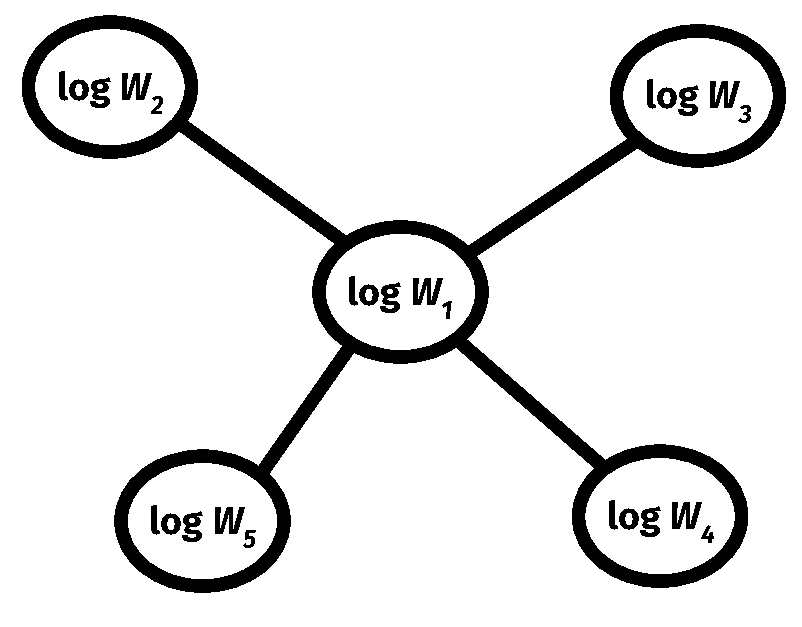
\includegraphics[width=110px]{figs/graph-model-log.pdf}
\end{center}
\end{column}
\end{columns}
\end{frame}

%\begin{frame}{Graphical model inference using SPIEC-EASI}
%\begin{columns}
%\begin{column}{0.5\textwidth}
%\textbf{If} we observed $\log W$\textellipsis
%\begin{center}
%$\widehat{\Omega} \rightarrow \widehat{\Omega^{-1}}$
%\end{center}
%\textbf{Instead}, we observe
%\begin{equation*}
%W\ \times\ ? \rightarrow \log W\ +\ ?
%\end{equation*}
%\textbf{Centered log-ratio (clr)} transformation eliminates \\ unknown constant by \\ centering each sample
%\end{column}
%\begin{column}{0.5\textwidth}
%\textbf{SPIEC-EASI}:
%\begin{center}
%Make OTU counts positive \\
%$\downarrow$ \\
%Centered log-ratio transformation \\
%$\downarrow$ \\
%Estimate $\Gamma = \cov(\clr W)$ and assume $\Gamma \approx \Omega$ \\
%$\downarrow$ \\
%Infer $\Omega^{-1}$ non-zero entries based on $\widehat{\Gamma}$
%\end{center}
%\end{column}
%\end{columns}
%\end{frame}

%\begin{frame}{Graphical model inference using SPIEC-EASI}
%\begin{equation*}
%\clr(x) = \left( \log \frac{x_1}{g(x)}, \dots, \log \frac{x_p}{g(x)} \right) = \left( \log x_1 - \frac{1}{p} \sum_{i=1}^p \log x_i, \dots \right)
%\end{equation*}
%\begin{center}
%\includegraphics[width=300px]{figs/clr.pdf}
%\end{center}
%\end{frame}

\begin{frame}{Covariance relationships and properties}
\textbf{Properties of $\Gamma$}
\begin{itemize}
\item $\gamma_{ij} = \omega_{ij} - \overline{\omega}_{i \cdot} - \overline{\omega}_{\cdot j} + \overline{\omega}_{\cdot \cdot}$
\item Rows/col's sum to zero
\item $p$ fewer free parameters than $\Omega$
\end{itemize}
\vspace{1em}
\pause
\begin{columns}
\begin{column}{0.45\textwidth}
$\Gamma \approx \Omega$
\begin{itemize}\begin{small}
\item Small or mostly negative correlations
\item Approx. equal variances
\item \textbf{Small \\ ``compositional effect"}
\end{small}\end{itemize}
\end{column}
\begin{column}{0.45\textwidth}
$\Gamma \not\approx \Omega$
\begin{itemize}\begin{small}
\item Mostly positive correlations
\item Unequal variances
\item \textbf{Large \\ ``compositional effect"}
\end{small}\end{itemize}
\end{column}
\end{columns}
\end{frame}

\begin{frame}{Covariance relationships and properties}
\textbf{One $\Gamma \leftrightarrow$ many $\Omega$}
\begin{center}
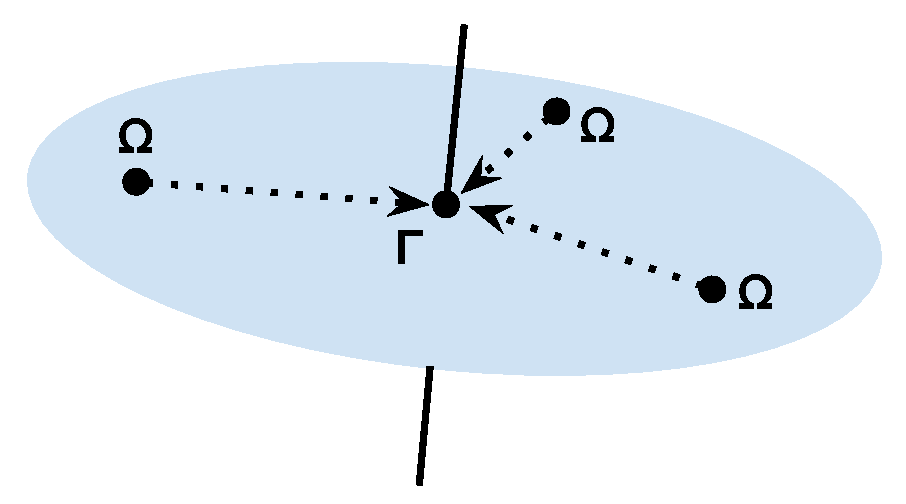
\includegraphics[width=200px]{figs/matrix-space.pdf}
\end{center}
\begin{itemize}
\item For each $\Gamma$, $p$-dimensional space of \textbf{potential $\Omega$s}
\end{itemize}
\end{frame}

\begin{frame}{Covariance relationships and properties}
\textbf{One $\Gamma \leftrightarrow$ many $\Omega$}
\begin{center}
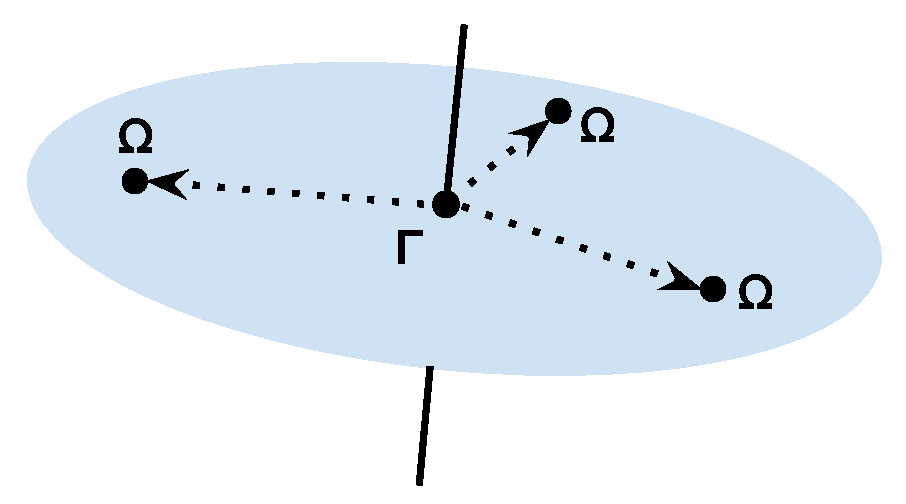
\includegraphics[width=200px]{figs/matrix-explore.pdf}
\end{center}
\begin{itemize}
\item Can solve for \textbf{potential $\Omega$s} (must check $\Omega \succ 0$)
\end{itemize}
\end{frame}

\begin{frame}{Covariance relationships and properties}
\textbf{Relationships can vary among potential $\Omega$s}
\begin{itemize}
\item Somewhat constrained, but not entirely
\end{itemize}
\textbf{Example} ($p = 24$, {\color{red} red} = negative, {\color{blue} blue} = positive)
\begin{columns}
\begin{column}{0.45\textwidth}
\begin{center}
$\widehat{\Gamma}$ (correlations)
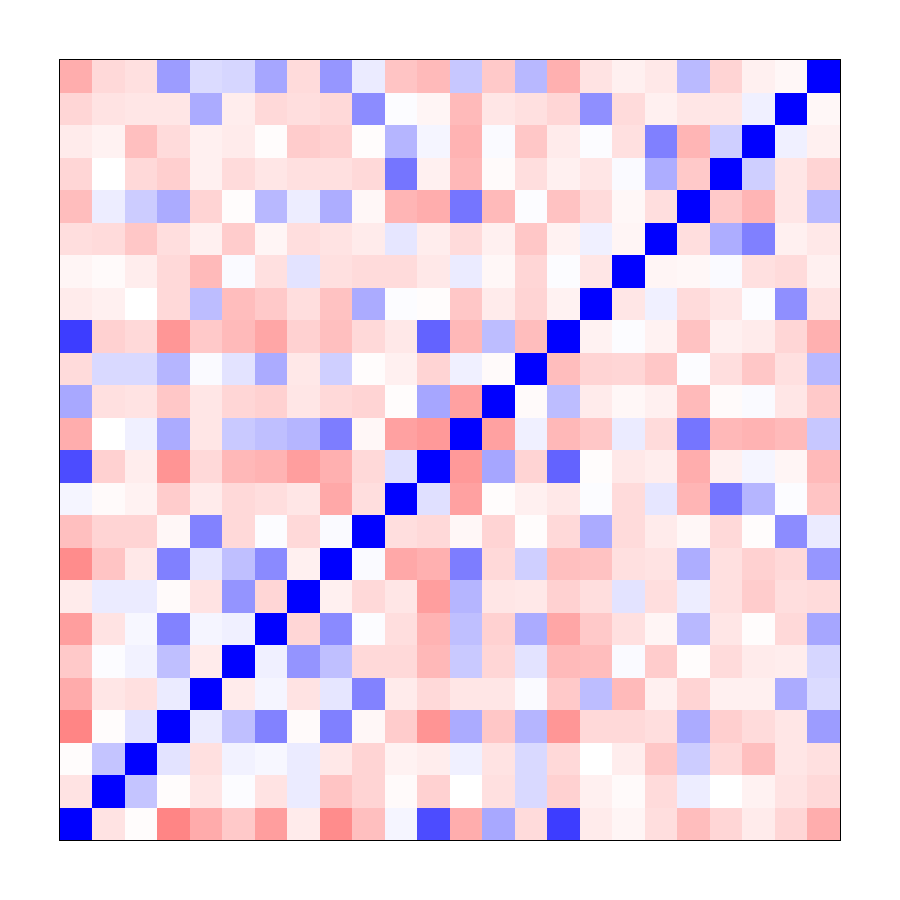
\includegraphics[width=90px]{figs/example-clr-cor.pdf}
\end{center}
\end{column}
\begin{column}{0.45\textwidth}
\begin{center}
Graph (24 edges)
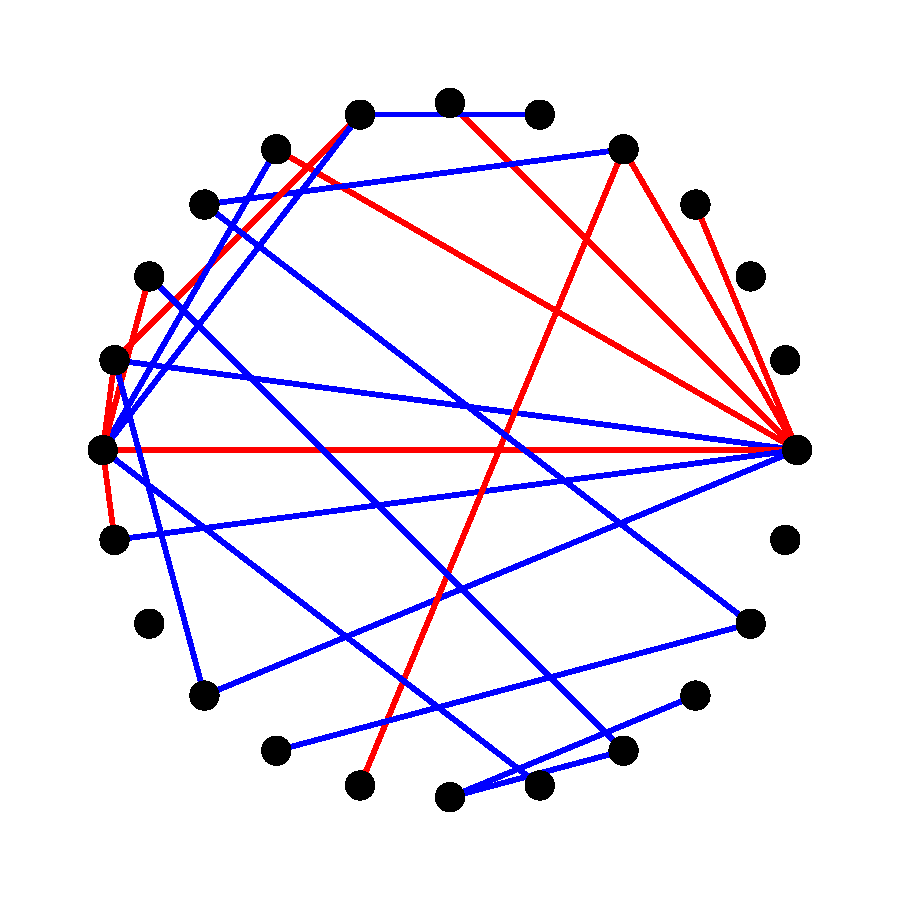
\includegraphics[width=90px]{figs/example-clr-graph.pdf}
\end{center}
\end{column}
\end{columns}
\end{frame}

\begin{frame}{Covariance relationships and properties}
\textbf{Relationships can vary among potential $\Omega$s}
\begin{itemize}
\item Somewhat constrained, but not entirely
\end{itemize}
\textbf{Example} ($p = 24$, {\color{red} red} = negative, {\color{blue} blue} = positive)
\begin{columns}
\begin{column}{0.45\textwidth}
\begin{center}
Potential $\widehat{\Omega}$ \#1
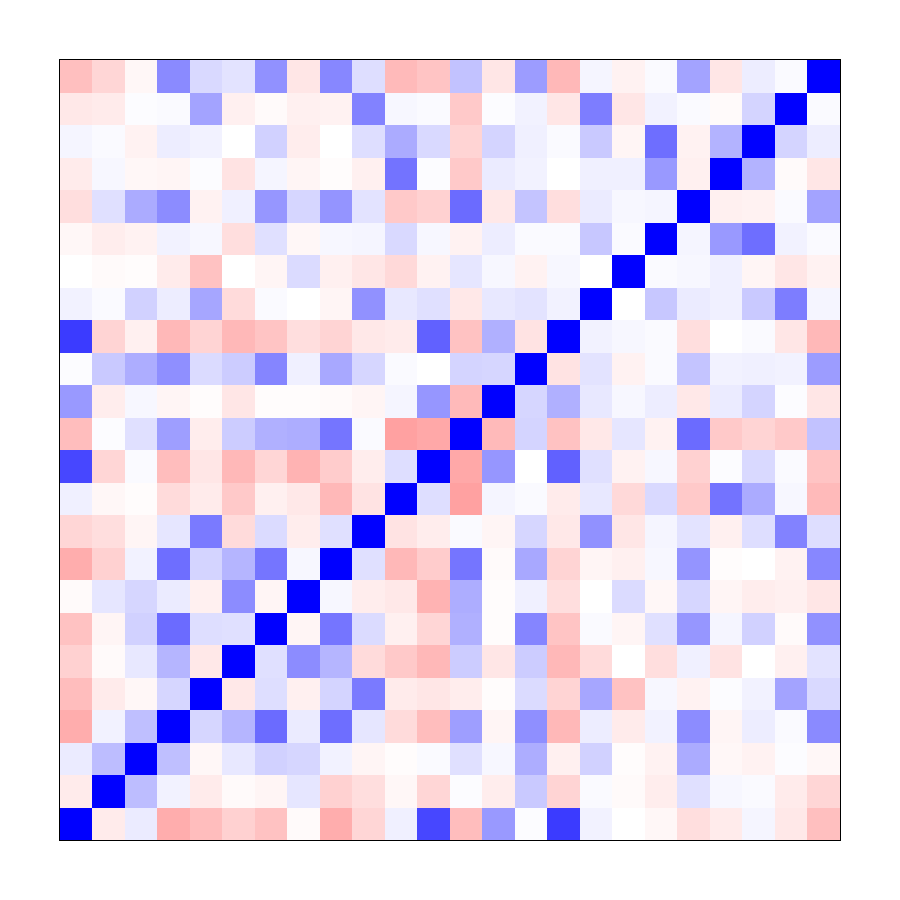
\includegraphics[width=90px]{figs/example-alt1-cor.pdf}
\end{center}
\end{column}
\begin{column}{0.45\textwidth}
\begin{center}
Graph (24 edges)
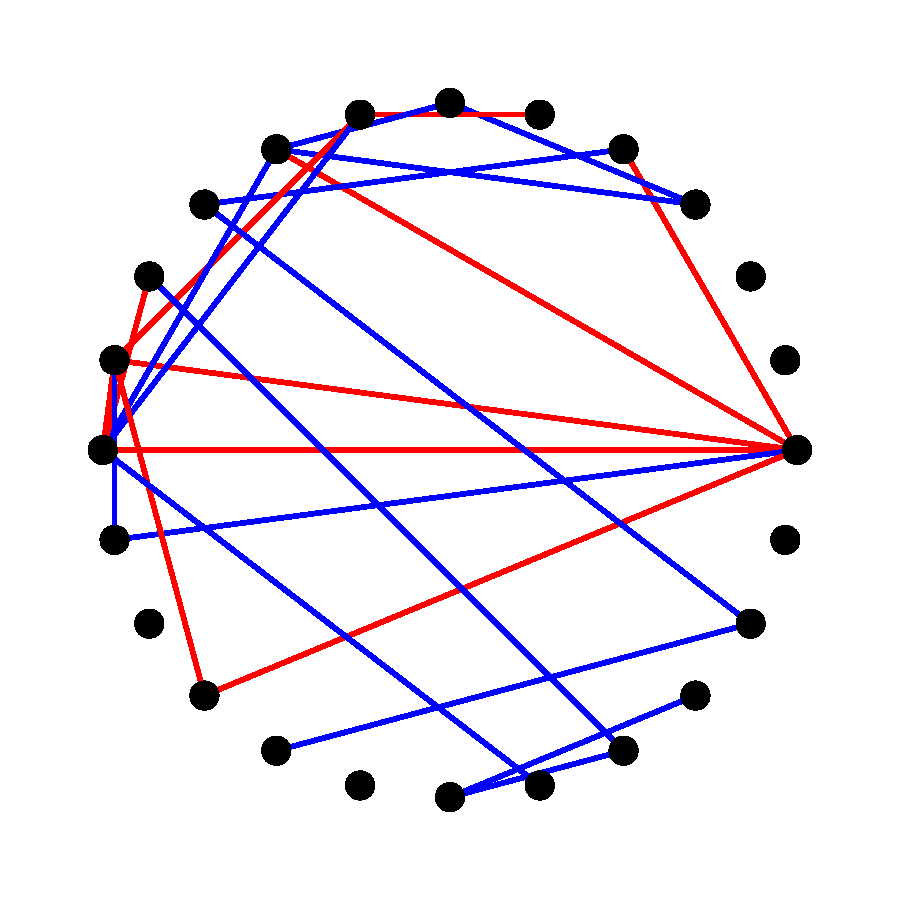
\includegraphics[width=90px]{figs/example-alt1-graph.pdf}
\end{center}
\end{column}
\end{columns}
\end{frame}

\begin{frame}{Covariance relationships and properties}
\textbf{Relationships can vary among potential $\Omega$s}
\begin{itemize}
\item Somewhat constrained, but not entirely
\end{itemize}
\textbf{Example} ($p = 24$, {\color{red} red} = negative, {\color{blue} blue} = positive)
\begin{columns}
\begin{column}{0.45\textwidth}
\begin{center}
Potential $\widehat{\Omega}$ \#2
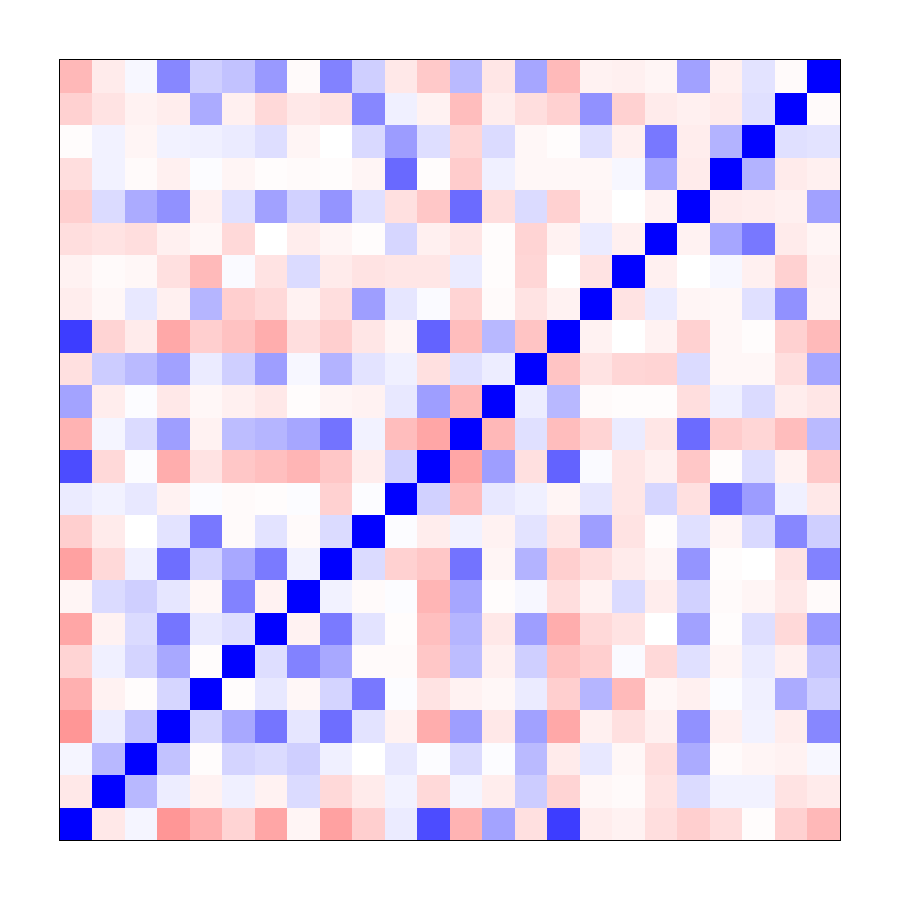
\includegraphics[width=90px]{figs/example-alt2-cor.pdf}
\end{center}
\end{column}
\begin{column}{0.45\textwidth}
\begin{center}
Graph (24 edges)
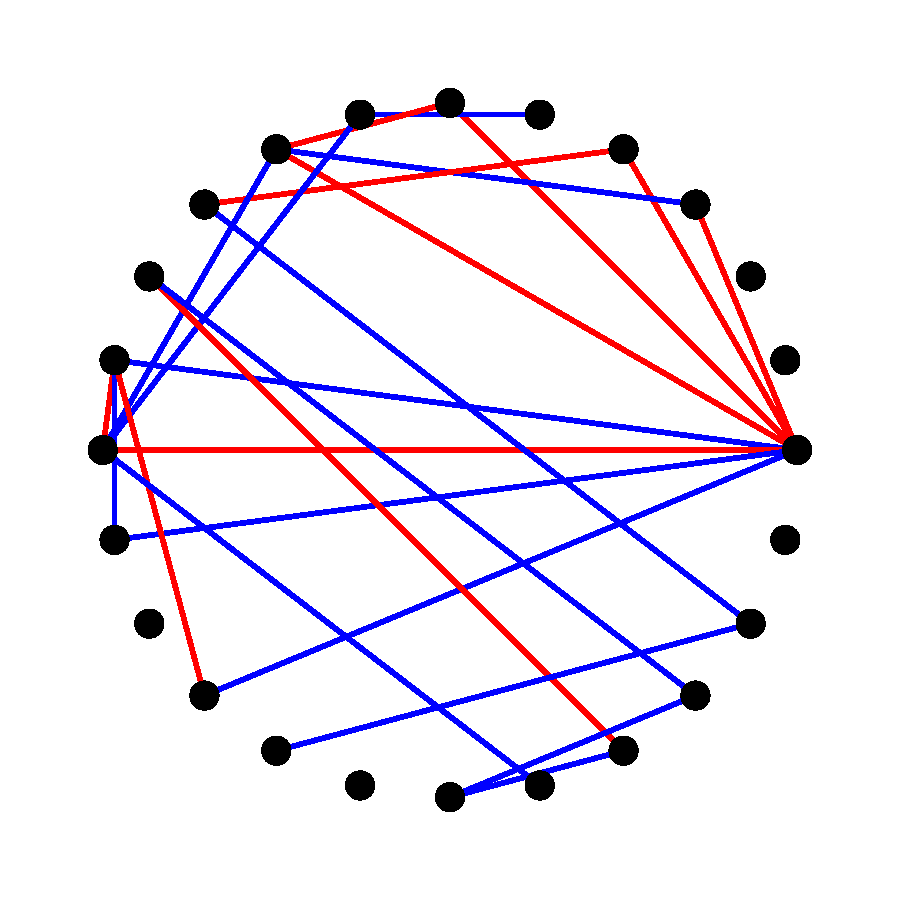
\includegraphics[width=90px]{figs/example-alt2-graph.pdf}
\end{center}
\end{column}
\end{columns}
\end{frame}

\begin{frame}{Covariance relationships and properties}
\textbf{Relationships can vary among potential $\Omega$s}
\begin{itemize}
\item Somewhat constrained, but not entirely
\end{itemize}
\textbf{Example} ($p = 24$, {\color{red} red} = negative, {\color{blue} blue} = positive)
\begin{columns}
\begin{column}{0.45\textwidth}
\begin{center}
Potential $\widehat{\Omega}$ \#3
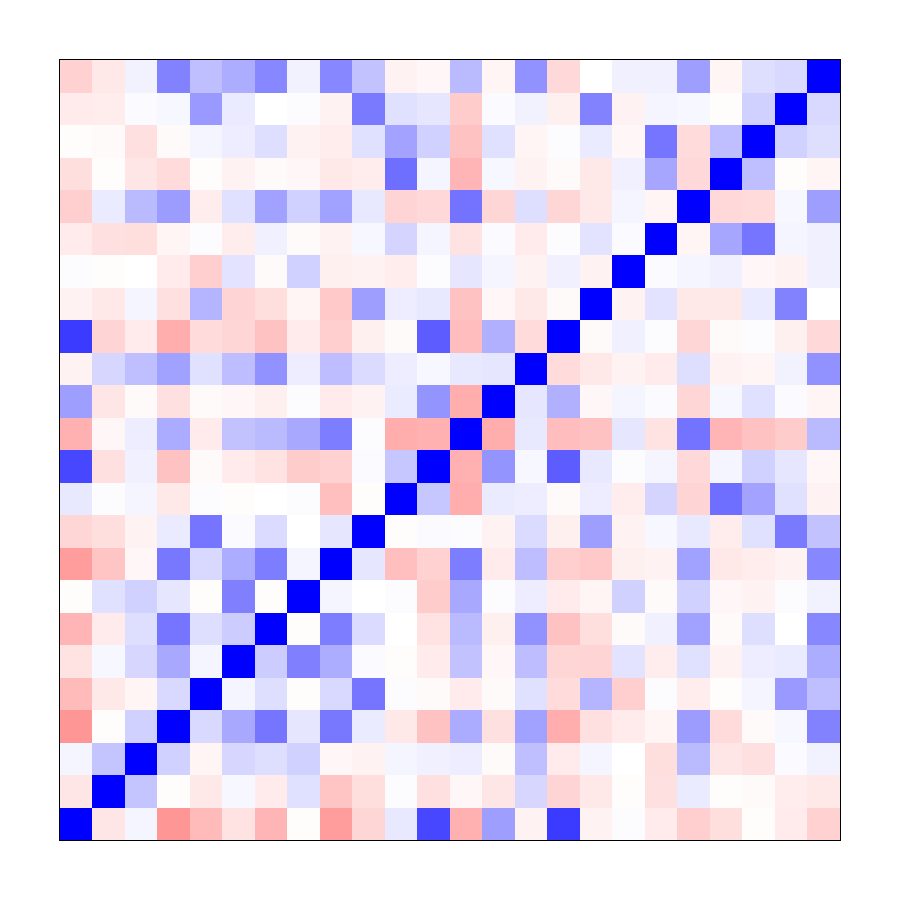
\includegraphics[width=90px]{figs/example-alt3-cor.pdf}
\end{center}
\end{column}
\begin{column}{0.45\textwidth}
\begin{center}
Graph (24 edges)
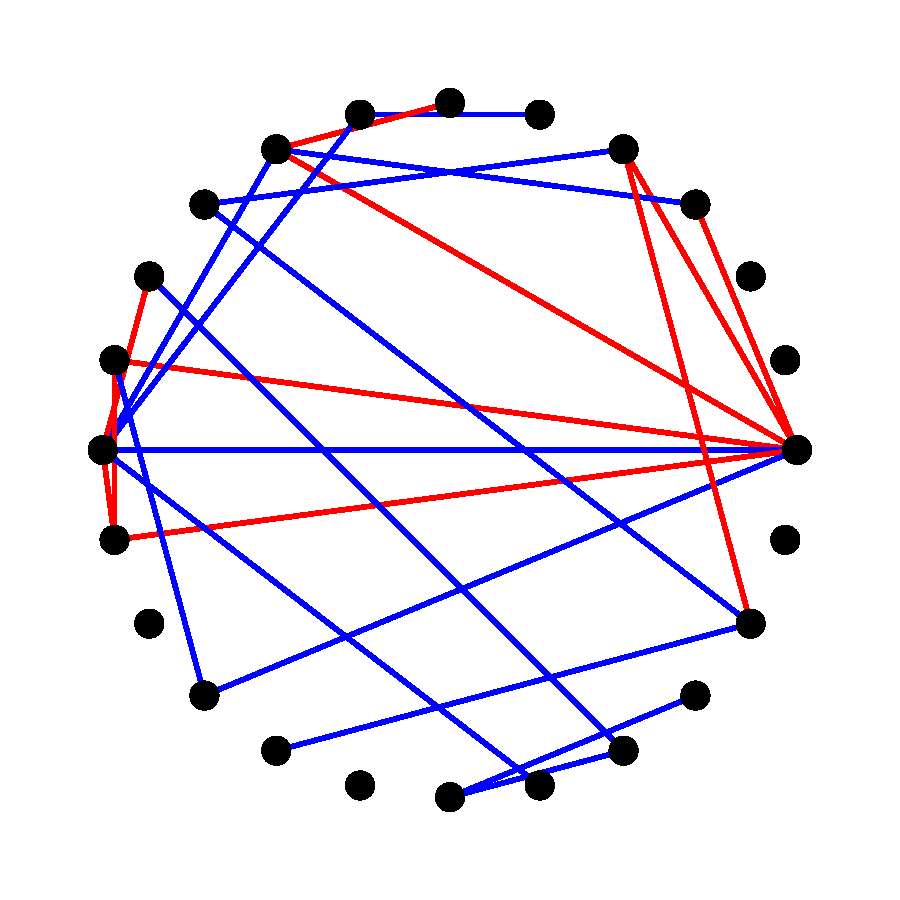
\includegraphics[width=90px]{figs/example-alt3-graph.pdf}
\end{center}
\end{column}
\end{columns}
\end{frame}

\begin{frame}{Graph selection performance}
Performance with \textbf{small compositional effect}
\begin{itemize}
\item Comparable to graph selection from log data
\end{itemize}
\begin{columns}
\begin{column}{0.6\textwidth}
\begin{center}
$p = 64$ \\
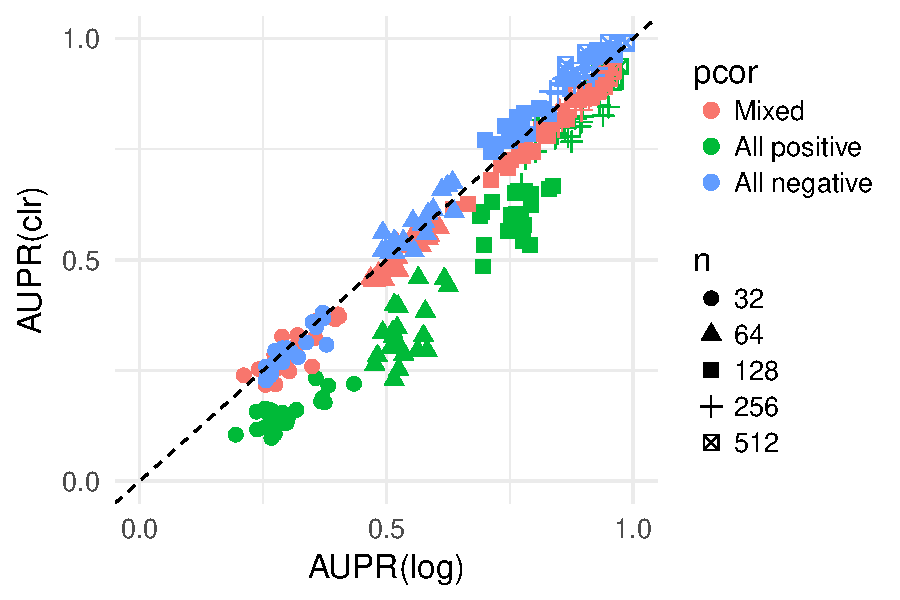
\includegraphics[width=210px]{figs/scalefree-aupr-64.pdf}
\end{center}
\end{column}
\begin{column}{0.35\textwidth}
\begin{small}
\begin{itemize}
\item Sparse graph
\item Approx. equal variances
\item Partial correlations (pcor) $\pm 0.25$
\item AUPR = area under precision-recall curve
\end{itemize}
\end{small}
\end{column}
\end{columns}
\end{frame}

\begin{frame}{Graph selection performance}
Performance with \textbf{small compositional effect}
\begin{itemize}
\item Comparable to graph selection from log data
\end{itemize}
\begin{columns}
\begin{column}{0.6\textwidth}
\begin{center}
$p = 256$ \\
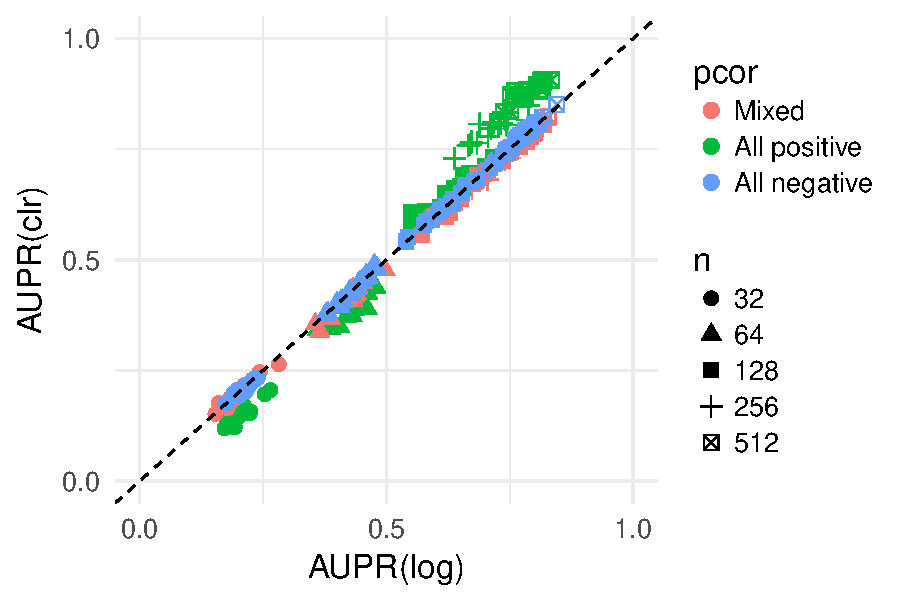
\includegraphics[width=210px]{figs/scalefree-aupr-256.pdf}
\end{center}
\end{column}
\begin{column}{0.35\textwidth}
\begin{small}
\begin{itemize}
\item Sparse graph
\item Approx. equal variances
\item Partial correlations (pcor) $\pm 0.25$
\item AUPR = area under precision-recall curve
\end{itemize}
\end{small}
\end{column}
\end{columns}
\end{frame}

\begin{frame}{Graph selection performance}
Performance with \textbf{large compositional effect}
\begin{itemize}
\item Affected by distortion of covariances
\end{itemize}
\begin{columns}
\begin{column}{0.6\textwidth}
\begin{center}
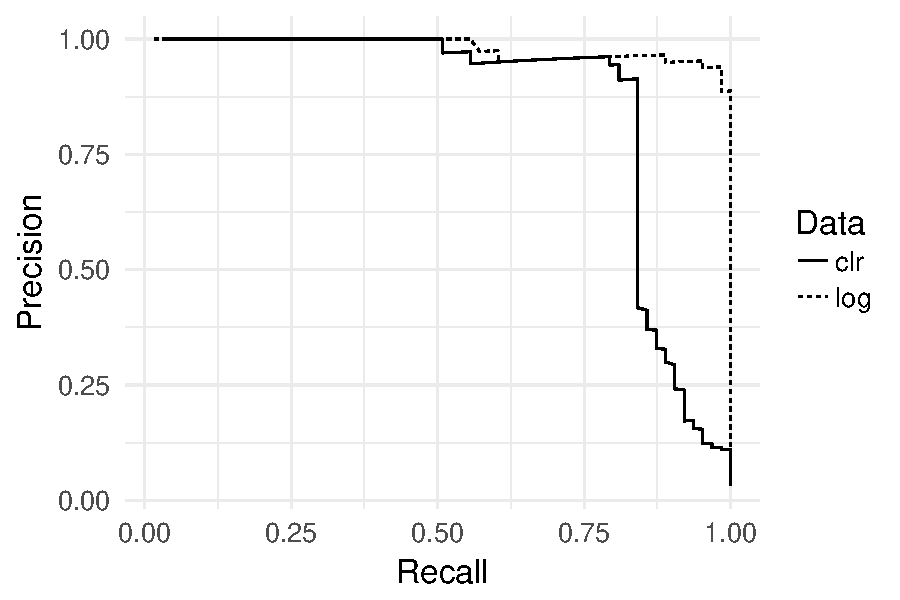
\includegraphics[width=210px]{figs/cluster-pr.pdf}
\end{center}
\end{column}
\begin{column}{0.35\textwidth}
\begin{small}
\begin{itemize}
\item Cluster graph, $p = 64$
\item $25\times$ larger variances in \\ one cluster
\item $n = 1024$
\end{itemize}
\end{small}
\end{column}
\end{columns}
\end{frame}

\begin{frame}{Graph selection performance}
Performance with \textbf{large compositional effect}
\begin{itemize}
\item Affected by distortion of covariances
\end{itemize}
\begin{center}
\begin{tabular}{ccc}
Graph & Data = log & Data = clr \\
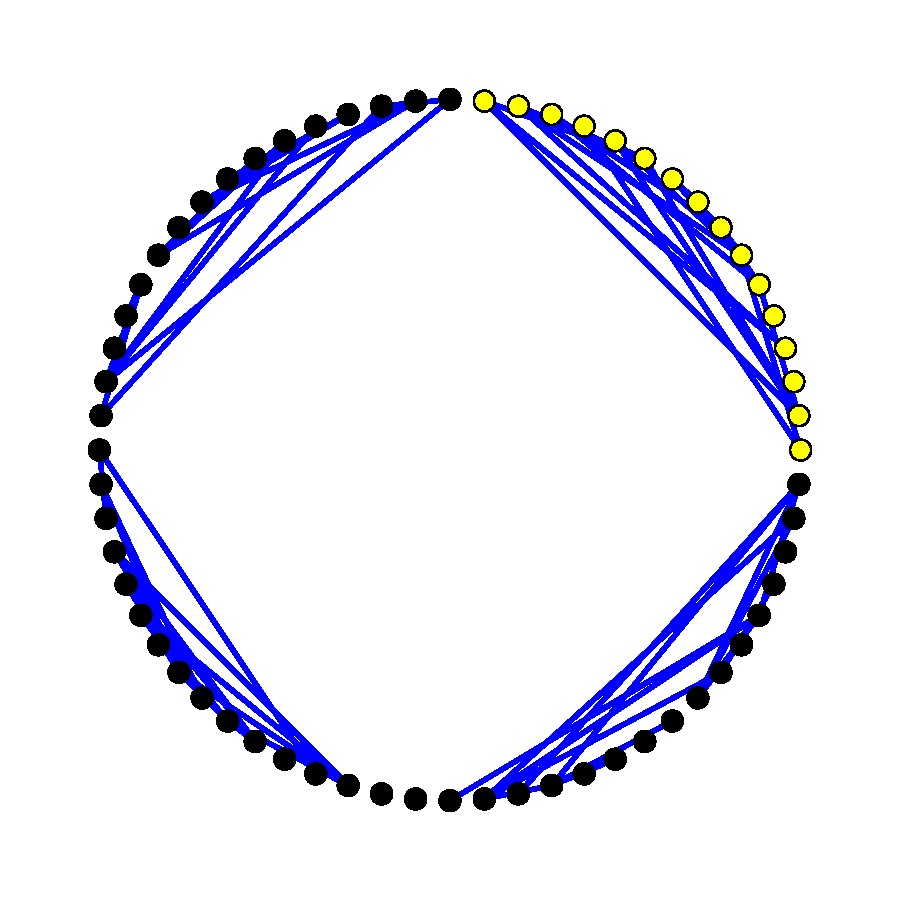
\includegraphics[width=90px]{figs/cluster-graph.pdf} &
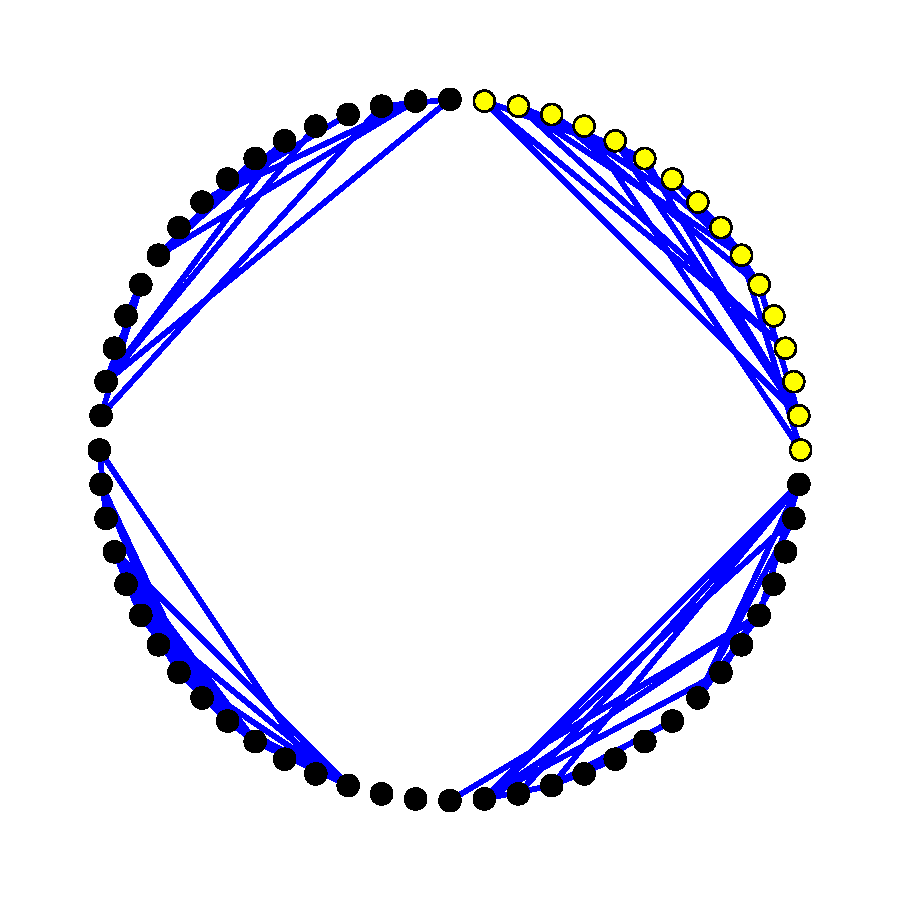
\includegraphics[width=90px]{figs/cluster-log.pdf} &
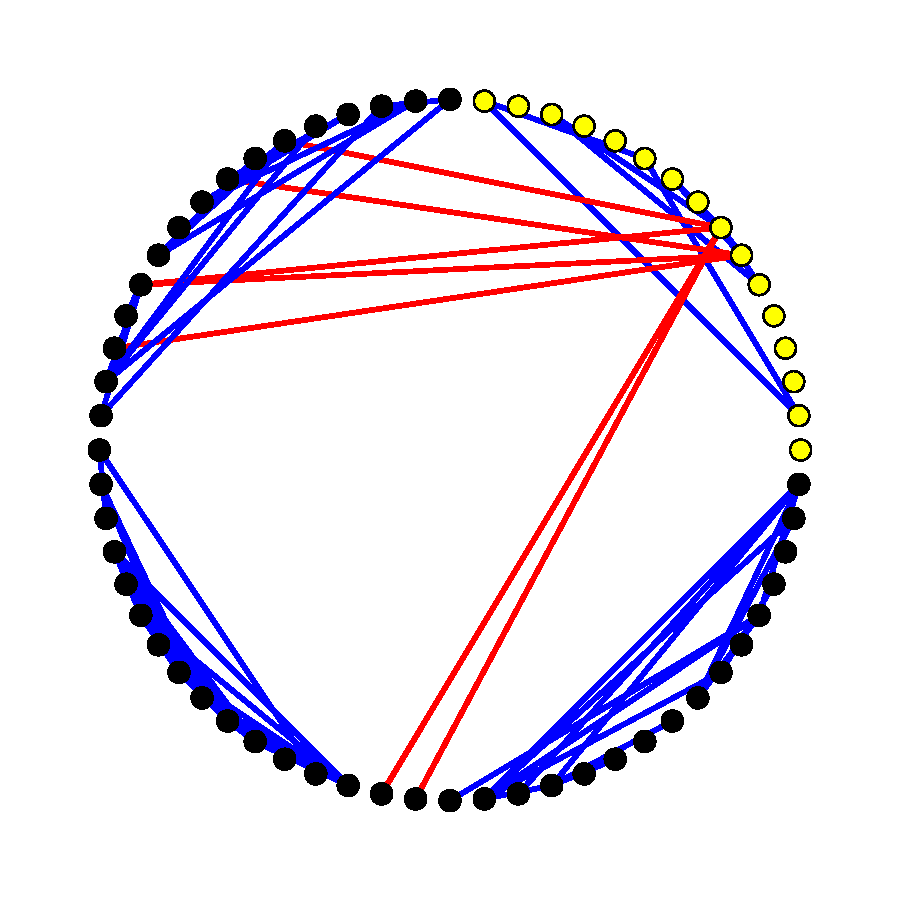
\includegraphics[width=90px]{figs/cluster-clr.pdf}
\end{tabular}
\vspace{3em}
\end{center}
\end{frame}

\begin{frame}{Summary}
\begin{itemize}
\item \textbf{Limitation of compositional data}: One $\Gamma \leftrightarrow$ many $\Omega$, uncertainty about $\log W$ relationships
\item \textbf{SPIEC-EASI graph selection} for $\log W$ \\ based on $\clr W$ data \textbf{performs well} \textellipsis \\ provided the compositional effect is not too large
\item \textbf{Large compositional effect} distorts covariances and causes erroneous edges in graph
\end{itemize}
\end{frame}

\begin{frame}{References \& Acknowledgements}
\textbf{SPIEC-EASI paper:}
\begin{itemize}
\item Kurtz., Z. D., M{\"u}ller, C. L., Miraldi, E. R., Littman, D. R., Blaser, M. J., and Bonneau, R. A. (2015). Sparse and compositionally robust inference of microbial ecological networks. \textit{PLoS Computational Biology} 11, e1004226.
\end{itemize}

\textbf{Thank you} Oregon State University faculty:
\begin{itemize}
\item Yuan Jiang, Duo Jiang, Sarah Emerson (Statistics)
\item Thomas Sharpton (Microbiology and Statistics)
\end{itemize}
\end{frame}

\appendix

\begin{frame}{Centered log-ratio transformation}
Given sample $x = (x_1, \dots, x_p)$ with geometric mean $g(x) = (\prod_{i=1}^p x_i)^{\frac{1}{p}}$,
\begin{align*}
\clr(x) &= \left( \log \frac{x_1}{g(x)}, \dots, \log \frac{x_p}{g(x)} \right) \\
&= \left( \log x_1 - \frac{1}{p} \sum_{i=1}^p \log x_i, \dots, \log x_p - \frac{1}{p} \sum_{i=1}^p \log x_i \right)
\end{align*}
and for $c > 0$,
\begin{equation*}
\clr(cx) = \clr(x)
\end{equation*}
\end{frame}

\begin{frame}{Covariance relationships}
\textbf{Matrix form}:
\begin{align*}
\clr W &= \text{G} \log W \\
\text{G} &=
\begin{pmatrix}
1-\frac{1}{p} & \dots & -\frac{1}{p} \\
\vdots & \ddots & \vdots \\
-\frac{1}{p} & \dots & 1-\frac{1}{p}
\end{pmatrix} \\
\Rightarrow \cov(\clr W) &= \text{G} \cov(\log W) \text{G} \\
\Rightarrow \Gamma &= \text{G} \Omega \text{G}
\end{align*}
\end{frame}

\begin{frame}{Graphical lasso estimation of $\Omega^{-1}$}
\begin{align*}
\widehat{\Omega^{-1}}_{\text{glasso}} &= \argmax_{\Omega^{-1} \succeq 0} \left[ \log \det(\Omega^{-1}) - \tr({\color{blue} \widehat{\Omega}} \Omega^{-1}) - \lambda \lVert \Omega^{-1} \rVert_1 \right] \\
\widehat{\Omega^{-1}}_{\text{SPIEC-EASI}} &= \argmax_{\Omega^{-1} \succeq 0} \left[ \log \det(\Omega^{-1}) - \tr({\color{blue} \widehat{\Gamma}} \Omega^{-1}) - \lambda \lVert \Omega^{-1} \rVert_1 \right]
\end{align*}
\end{frame}

\begin{frame}{Solving for potential $\Omega$}
\textbf{Option 1}: Choose $\overline{\omega}_{1\cdot}, \dots, \overline{\omega}_{p\cdot}$
\begin{align*}
\gamma_{ij} &= \omega_{ij} - \overline{\omega}_{i \cdot} - \overline{\omega}_{\cdot j} + \overline{\omega}_{\cdot \cdot} \\
\Rightarrow \omega_{ij} &= \gamma_{ij} + \overline{\omega}_{i \cdot} + \overline{\omega}_{\cdot j} - \overline{\omega}_{\cdot \cdot}
\end{align*}
\textbf{Option 2}: Choose $\omega_{11}, \dots, \omega_{pp}$
\begin{equation*}
\omega_{ij} = \gamma_{ij} + \frac{1}{2}\left( \omega_{ii} - \gamma_{ii} + \omega_{jj} - \gamma_{jj}\right)
\end{equation*}
\end{frame}

\begin{frame}{Graphs used in simulations}
$p = 64$, $e = p - 1$
\begin{center}
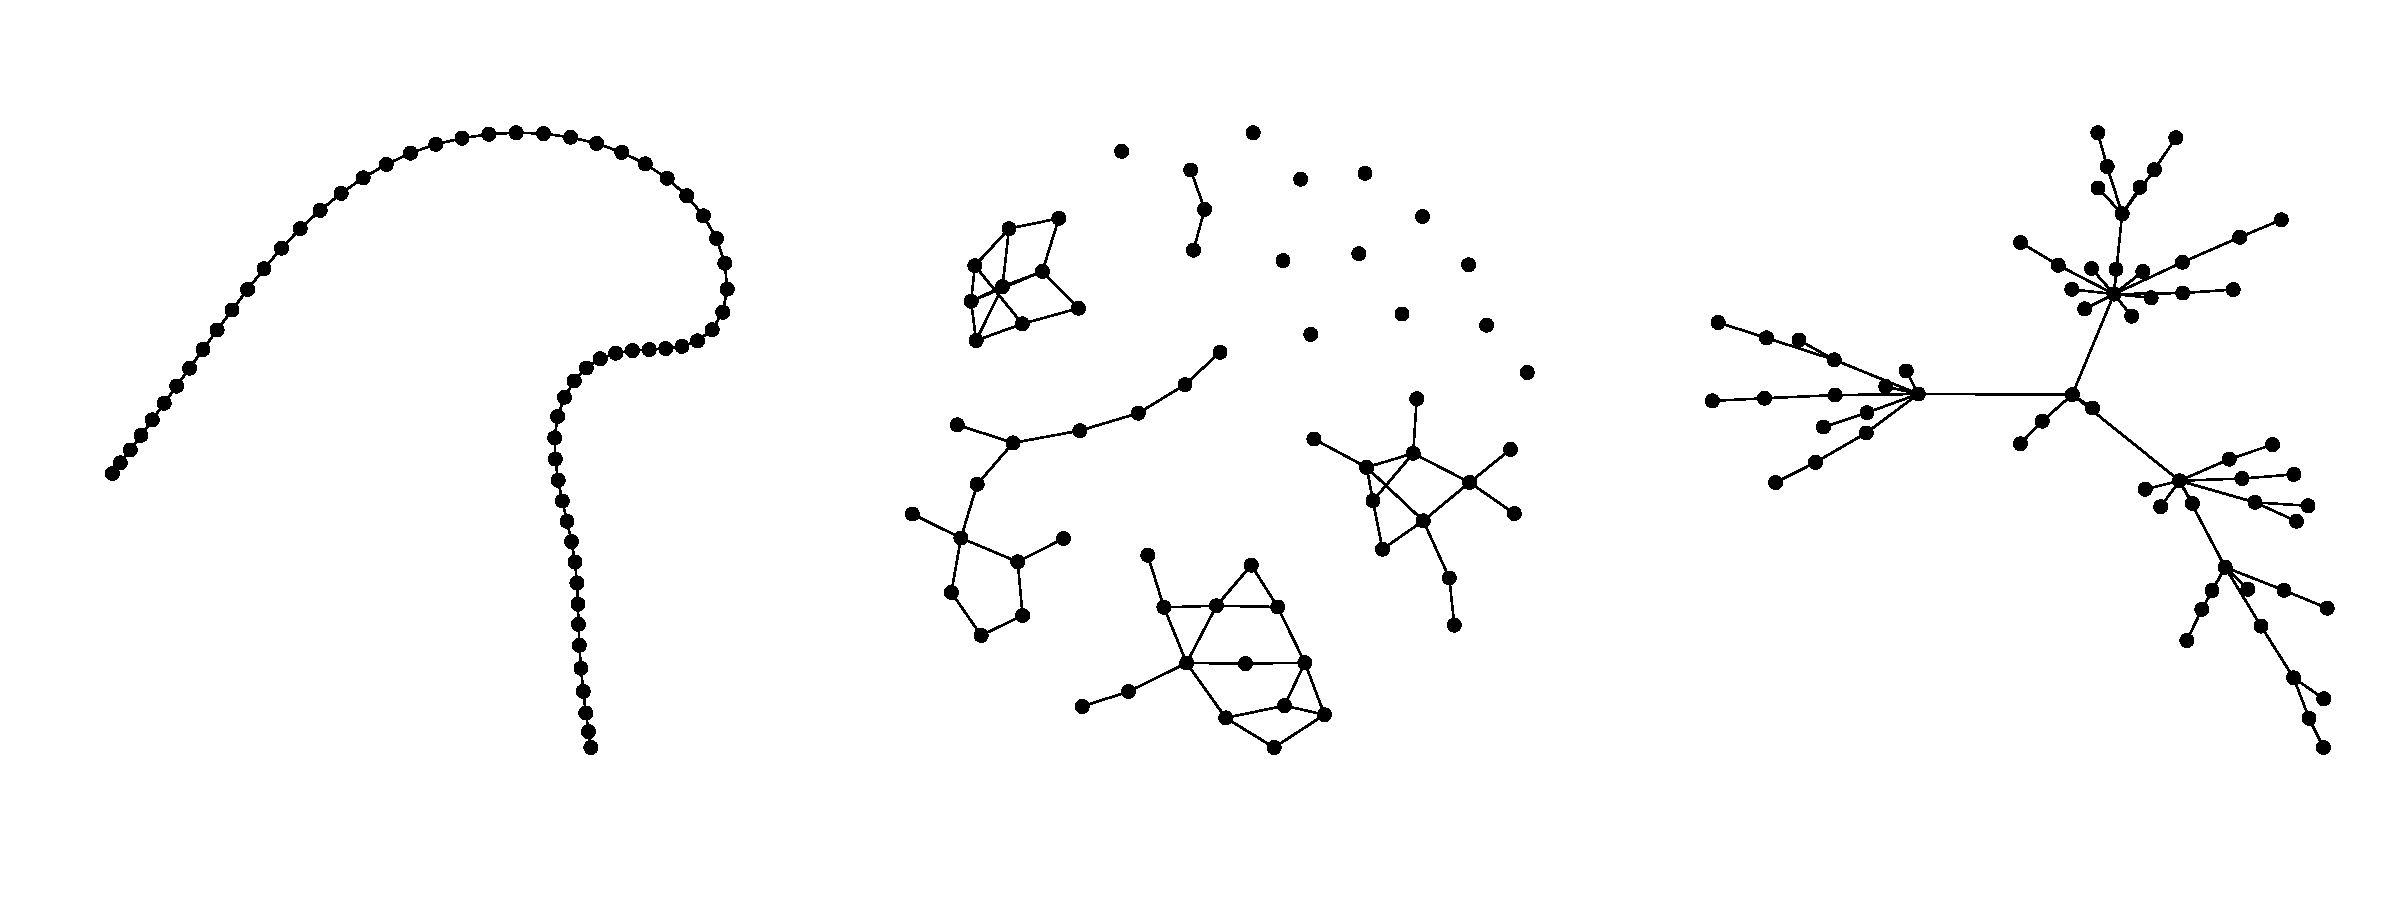
\includegraphics[width=300px]{figs/graphs-64.pdf}
\end{center}
\begin{columns}
\begin{column}{0.3\textwidth}
\centering Band
\end{column}
\begin{column}{0.3\textwidth}
\centering Cluster
\end{column}
\begin{column}{0.3\textwidth}
\centering Scale-free
\end{column}
\end{columns}
\end{frame}
\end{document}